\documentclass[tikz,border=8pt]{standalone}
\usepackage[T1]{fontenc}
\usepackage{lmodern}
\usepackage{tikz}
\usetikzlibrary{arrows.meta,calc,decorations.pathreplacing,fit,matrix,positioning}

\definecolor{cornellred}{HTML}{B31B1B}
\definecolor{ink}{HTML}{202124}
\definecolor{muted}{HTML}{667085}
\definecolor{line}{HTML}{AEB8C6}
\definecolor{paper}{HTML}{FFFFFF}
\definecolor{soft}{HTML}{F5F7FA}
\definecolor{camera}{HTML}{E8F4FF}
\definecolor{memory}{HTML}{F0F7EC}
\definecolor{compute}{HTML}{FFF3E6}
\definecolor{display}{HTML}{F7ECF3}
\definecolor{verify}{HTML}{EFEAFE}

\tikzset{
  font=\sffamily,
  flow/.style={
    -{Latex[length=2.6mm,width=1.8mm]},
    draw=muted,
    line width=0.8pt,
    rounded corners=2pt
  },
  dataflow/.style={
    flow,
    draw=cornellred
  },
  block/.style={
    rectangle,
    rounded corners=3pt,
    draw=line,
    line width=0.8pt,
    fill=paper,
    align=center,
    minimum width=28mm,
    minimum height=10mm,
    inner xsep=4pt,
    inner ysep=4pt
  },
  smallblock/.style={
    block,
    minimum width=22mm,
    minimum height=8mm,
    font=\sffamily\scriptsize
  },
  title/.style={
    font=\sffamily\bfseries\large,
    text=ink
  },
  labeltext/.style={
    font=\sffamily\scriptsize,
    text=muted,
    align=center
  },
  camera_block/.style={block, fill=camera, draw=blue!45!black},
  memory_block/.style={block, fill=memory, draw=green!45!black},
  compute_block/.style={block, fill=compute, draw=orange!65!black},
  display_block/.style={block, fill=display, draw=purple!45!black},
  verify_block/.style={block, fill=verify, draw=violet!50!black},
  groupbox/.style={
    draw=line,
    rounded corners=5pt,
    line width=0.7pt,
    fill=soft,
    inner sep=7pt
  }
}


\begin{document}
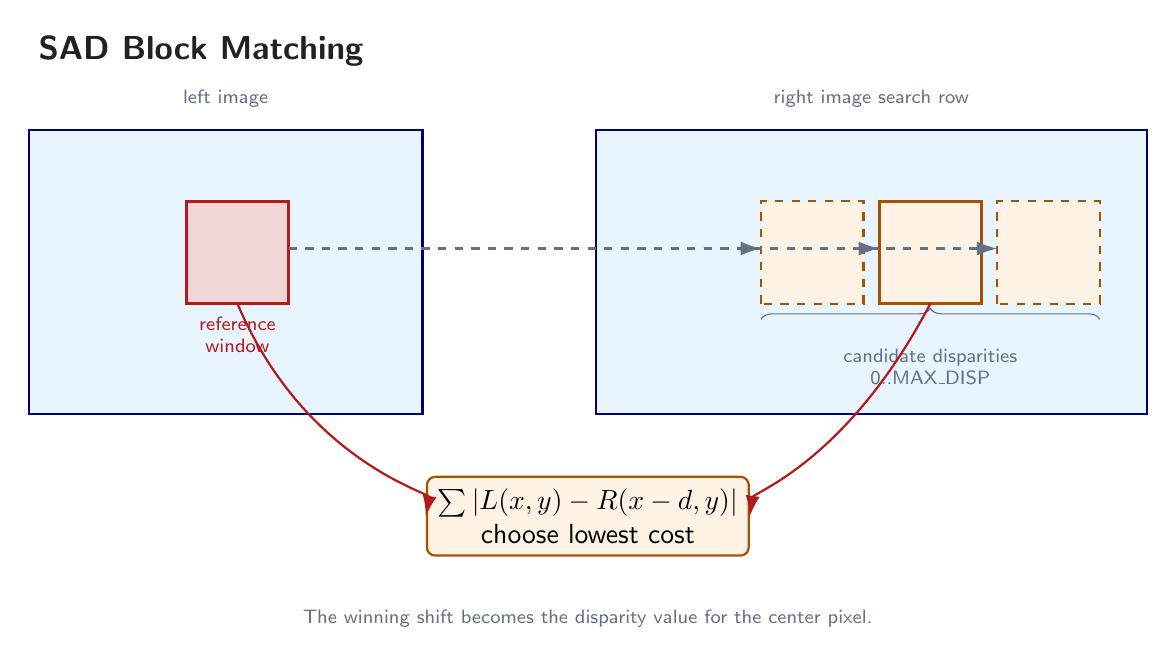
\begin{tikzpicture}[x=1mm,y=1mm]
  \node[title, anchor=west] at (0, 64) {SAD Block Matching};

  \draw[fill=camera, draw=blue!45!black, line width=0.8pt] (0,18) rectangle (50,54);
  \draw[fill=camera, draw=blue!45!black, line width=0.8pt] (72,18) rectangle (142,54);

  \node[labeltext] at (25,58) {left image};
  \node[labeltext] at (107,58) {right image search row};

  \draw[fill=cornellred!18, draw=cornellred, line width=1.2pt] (20,32) rectangle (33,45);
  \node[labeltext, text=cornellred] at (26.5,28) {reference\\window};

  \draw[fill=compute, draw=orange!65!black, line width=1pt] (108,32) rectangle (121,45);
  \draw[fill=compute, draw=orange!65!black, line width=0.8pt, dashed] (93,32) rectangle (106,45);
  \draw[fill=compute, draw=orange!65!black, line width=0.8pt, dashed] (123,32) rectangle (136,45);

  \draw[flow, dashed] (33,39) -- (93,39);
  \draw[flow, dashed] (33,39) -- (108,39);
  \draw[flow, dashed] (33,39) -- (123,39);

  \draw[decorate, decoration={brace, amplitude=4pt}, draw=muted] (93,30) -- (136,30);
  \node[labeltext] at (114.5,24) {candidate disparities\\0..MAX\_DISP};

  \node[compute_block, minimum width=38mm] (sad) at (71,5) {$\sum |L(x,y)-R(x-d,y)|$\\choose lowest cost};
  \draw[dataflow] (26.5,32) .. controls (35,12) and (51,8) .. (sad.west);
  \draw[dataflow] (114.5,32) .. controls (104,12) and (92,8) .. (sad.east);

  \node[labeltext, align=center] at (71,-8) {The winning shift becomes the disparity value for the center pixel.};
\end{tikzpicture}
\end{document}

